%%%%%%%%%%%%%%%%%%%%%%%%%%
%%% author : Yamada. T %%%
%%% made for TH series %%%
%%%%%%%%%%%%%%%%%%%%%%%%%%

\documentclass[b5paper,10pt,fleqn] {ltjsarticle}

\usepackage[margin=10truemm]{geometry}

\usepackage{pict2e, graphicx}
\usepackage{tikz}
\usetikzlibrary{intersections,calc,arrows.meta}

\usepackage{amsmath, amssymb, amsthm}
\usepackage{ascmac}
\usepackage{comment}
\usepackage{empheq}
\usepackage[shortlabels,inline]{enumitem}
\usepackage{fancybox}
\usepackage{fancyhdr}
\usepackage{here}
\usepackage{lastpage}
\usepackage{listings, jvlisting}
\usepackage{fixdif}

\usepackage{stmaryrd}
\usepackage[listings]{tcolorbox}
%\usepackage{ascolorbox}
\usepackage{titlesec}
\usepackage{ulem}
\usepackage{url}
\usepackage{verbatim}
\usepackage{wrapfig}
\usepackage{xcolor}
\usepackage{luatexja-ruby}
\usepackage{varwidth}
\usepackage[version=3]{mhchem}
\usepackage{wrapfig}


\usepackage{physics2}
	\usephysicsmodule{ab}
	\usephysicsmodule{ab.braket}
	\usephysicsmodule{ab.legacy}
	%\usephysicsmodule{braket}
	\usephysicsmodule{diagmat}
	\usephysicsmodule{xmat}
	\usephysicsmodule{nabla.legacy}
	\usephysicsmodule{qtext.legacy}

\usepackage[ISO]{diffcoeff}
\difdef { f, s } { D }
{ op-symbol = \mathrm{D} }


\newcommand{\mctext}[1]{\mbox{\textcircled{\scriptsize{#1}}}}
\newcommand{\ctext}[1]{\textcircled{\scriptsize{#1}}}
\newcommand{\ds}{\displaystyle}
\newcommand{\comb}[2]{{}_{#1}\mathrm{C}_{#2}}
\newcommand{\hs}{\hspace}
\newcommand{\vs}{\vspace}
\newcommand{\emphvs}{\vspace{1em}\notag\\}
\newcommand{\ora}{\overrightarrow}
\newcommand{\ol}{\overline}
\newcommand{\oramr}[1]{\overrightarrow{\mathrm{#1}}}
\newcommand{\tri}{\triangle}
\newcommand{\mr}{\mathrm}
\newcommand{\mb}{\mathbb}
\newcommand{\mrvec}[1]{\overrightarrow{\mathrm{#1}}}
\newcommand{\itvec}{\overrightarrow}
\newcommand{\bs}{\boldsymbol}
\newcommand{\ra}{\rightarrow}
\newcommand{\Ra}{\Rightarrow}
\newcommand{\lra}{\longrightarrow}
\newcommand{\Lra}{\Longrightarrow}
\newcommand{\la}{\leftarrow}
\newcommand{\La}{\Leftarrow}
\newcommand{\lla}{\longleftarrow}
\newcommand{\Lla}{\Longleftarrow}
\newcommand{\lr}{\leftrightarrow}
\newcommand{\llr}{\longleftrightarrow}
\newcommand{\Llr}{\Longleftrightarrow}
\renewcommand{\deg}{{}^\circ}
\newcommand{\phbox}{\fbox{\phantom{1\hspace{2em}}}}
\newcommand{\boxnum}[1]{\fbox{\phantom{\hspace{1em}}({#1})\phantom{\hspace{1em}}}}
\newcommand{\boxkana}[1]{\fbox{\phantom{\hspace{1em}}{#1}\phantom{\hspace{1em}}}}
\newcommand{\boxkm}[2]{\fbox{\, {#1}\phantom{\hspace{0.2em}} \,  {#2}}}
\newcommand{\hzw}{\hspace{1\zw}}

\renewcommand{\baselinestretch}{1.25}
\parindent=1\zw


%TH3-22

\setlist[enumerate]{labelsep=1\zw, itemindent=1\zw, listparindent=1\zw}

\begin{document}
\noindent\fbox{NewTH4-11} [東京大]

3つの電球,可変抵抗,電流計,電池(起電力4 V)およびスイッチを導線で接続し,図1に示す回路を作った.電球の電流・電圧特性は,スイッチを入れた直後ではオームの法則に従うが,十分に時間が経過すると図2の特性を示すものとする.
電流計と電池の内部抵抗は合わせて$r$〔$\Omega$〕で,スイッチを含め導線の抵抗は無視できるものとする.

\begin{minipage}[b]{0.45\linewidth}
  \begin{figure}[H]
    \centering
    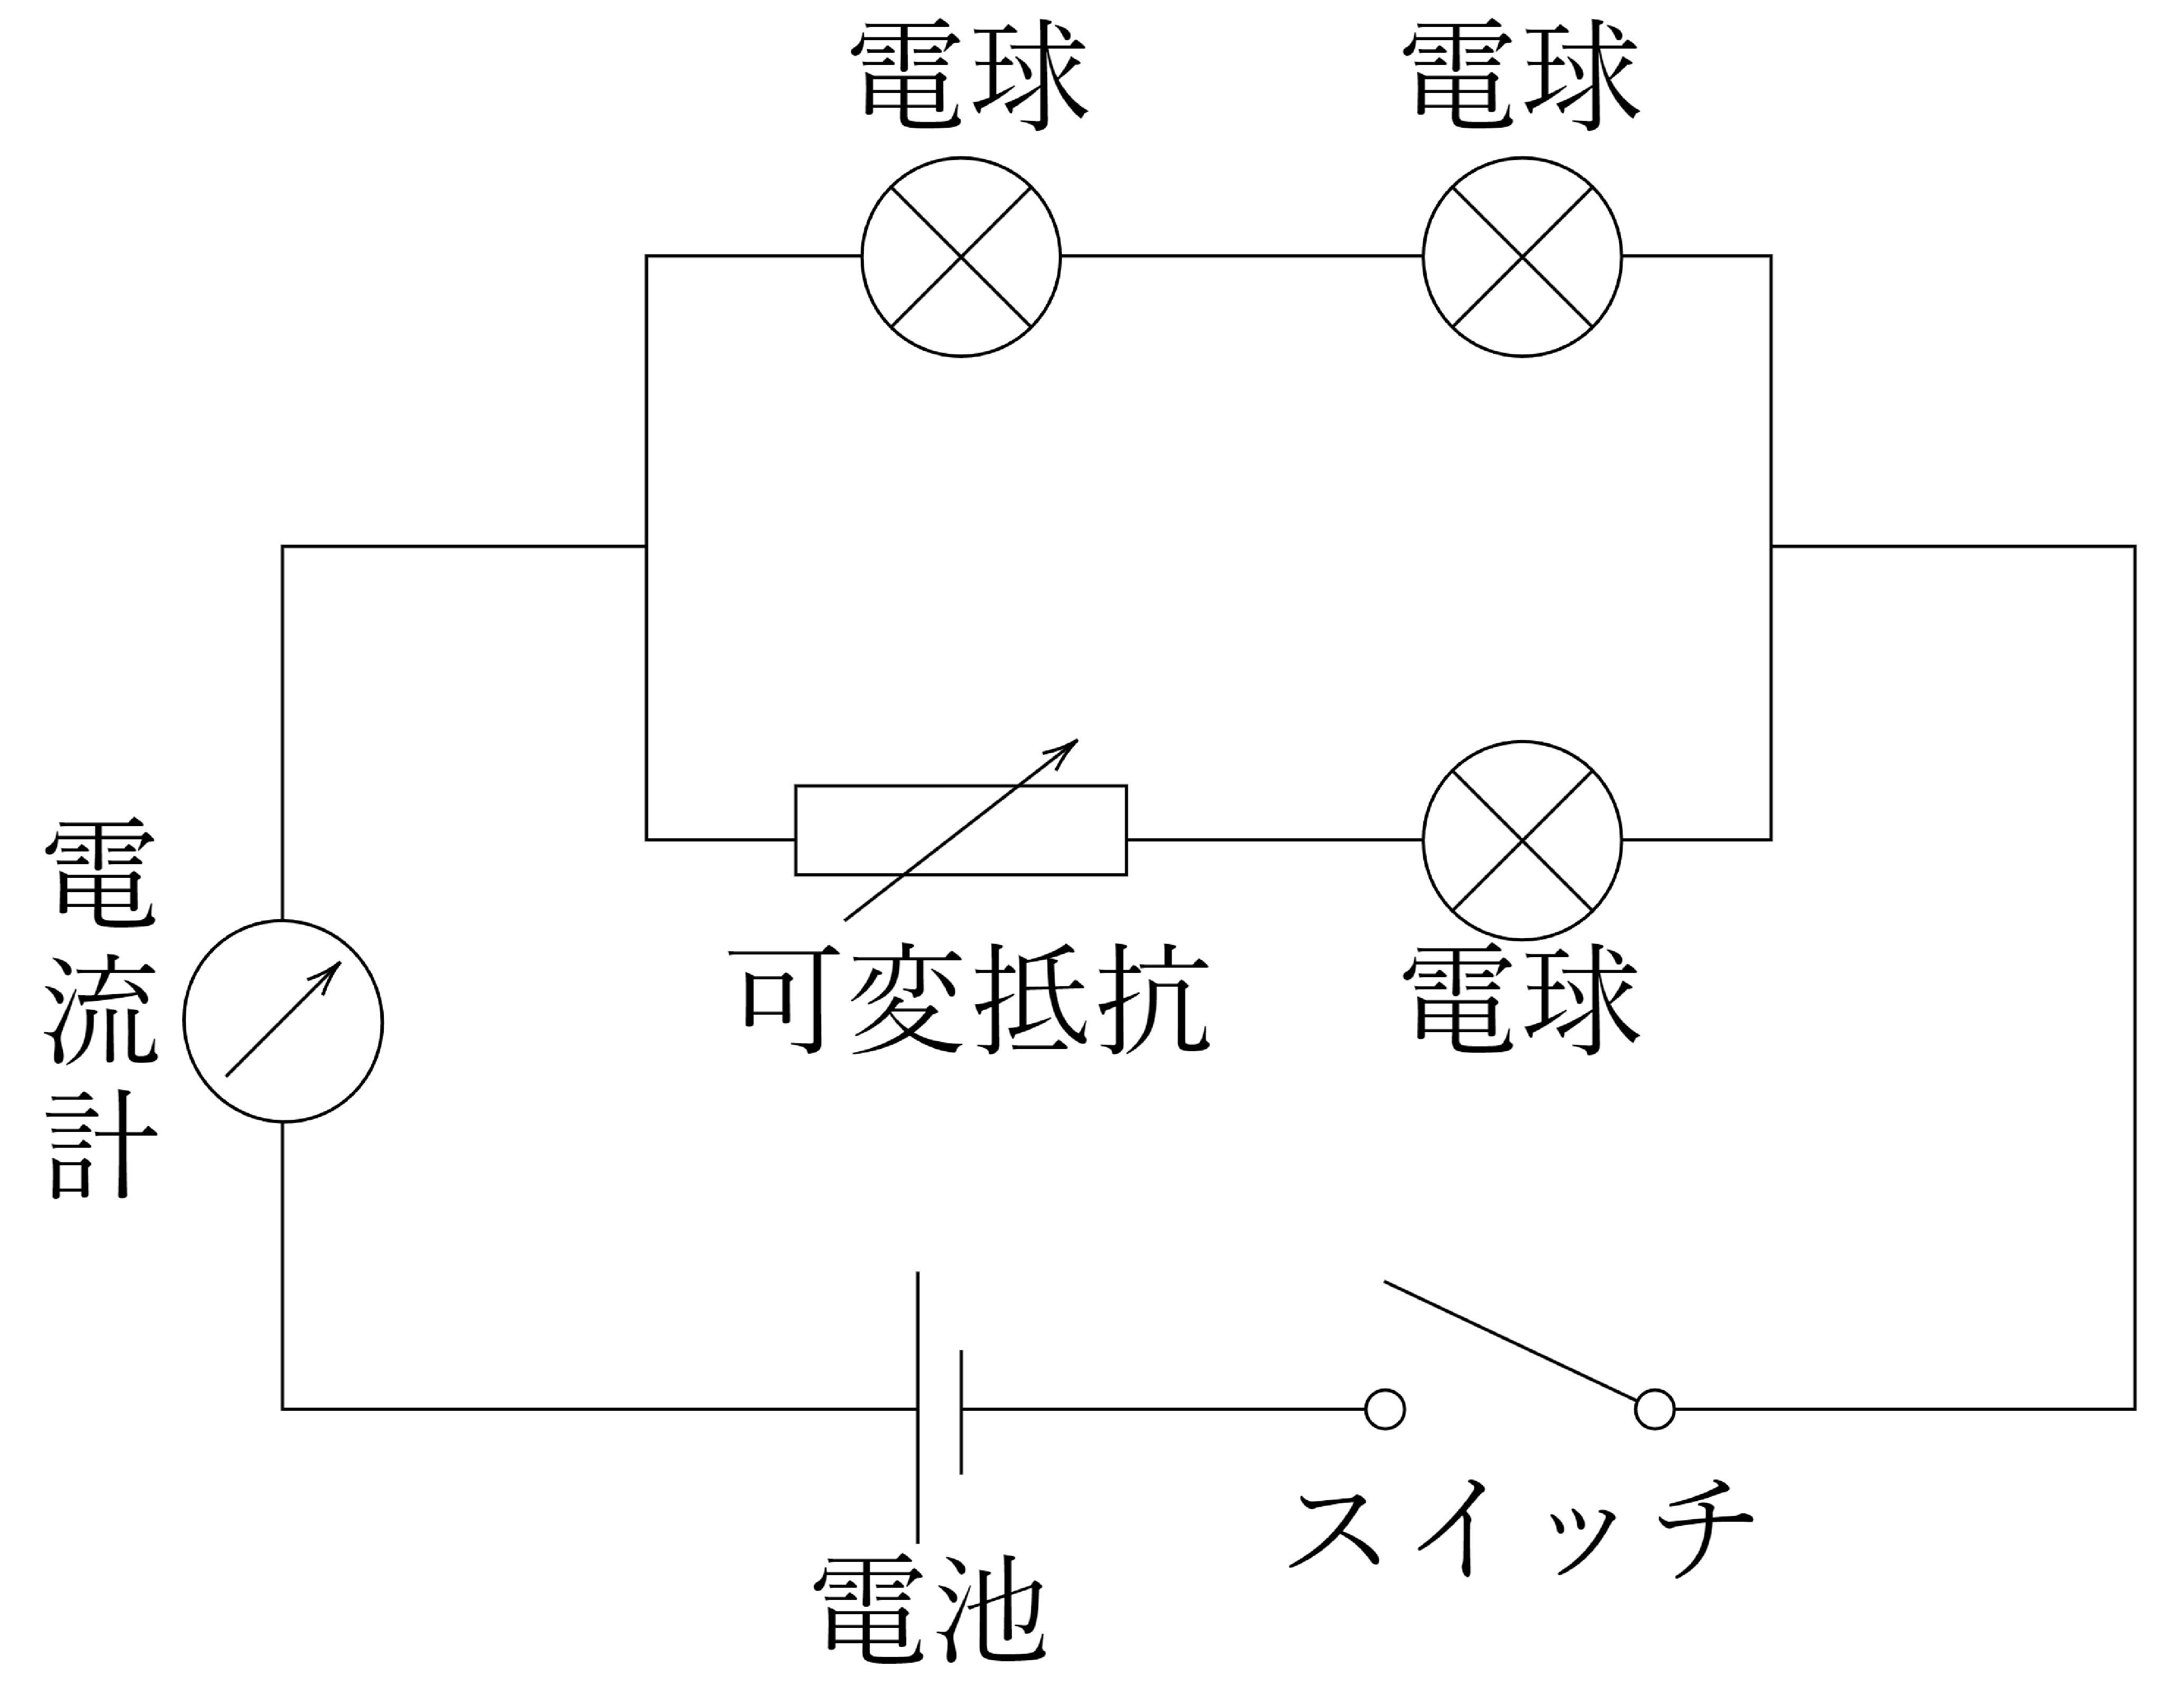
\includegraphics[width=6cm]{fig/fig_4_11_1.pdf}
    \caption{}
  \end{figure}
\end{minipage}
\begin{minipage}[b]{0.45\linewidth}
  \begin{figure}[H]
    \centering
    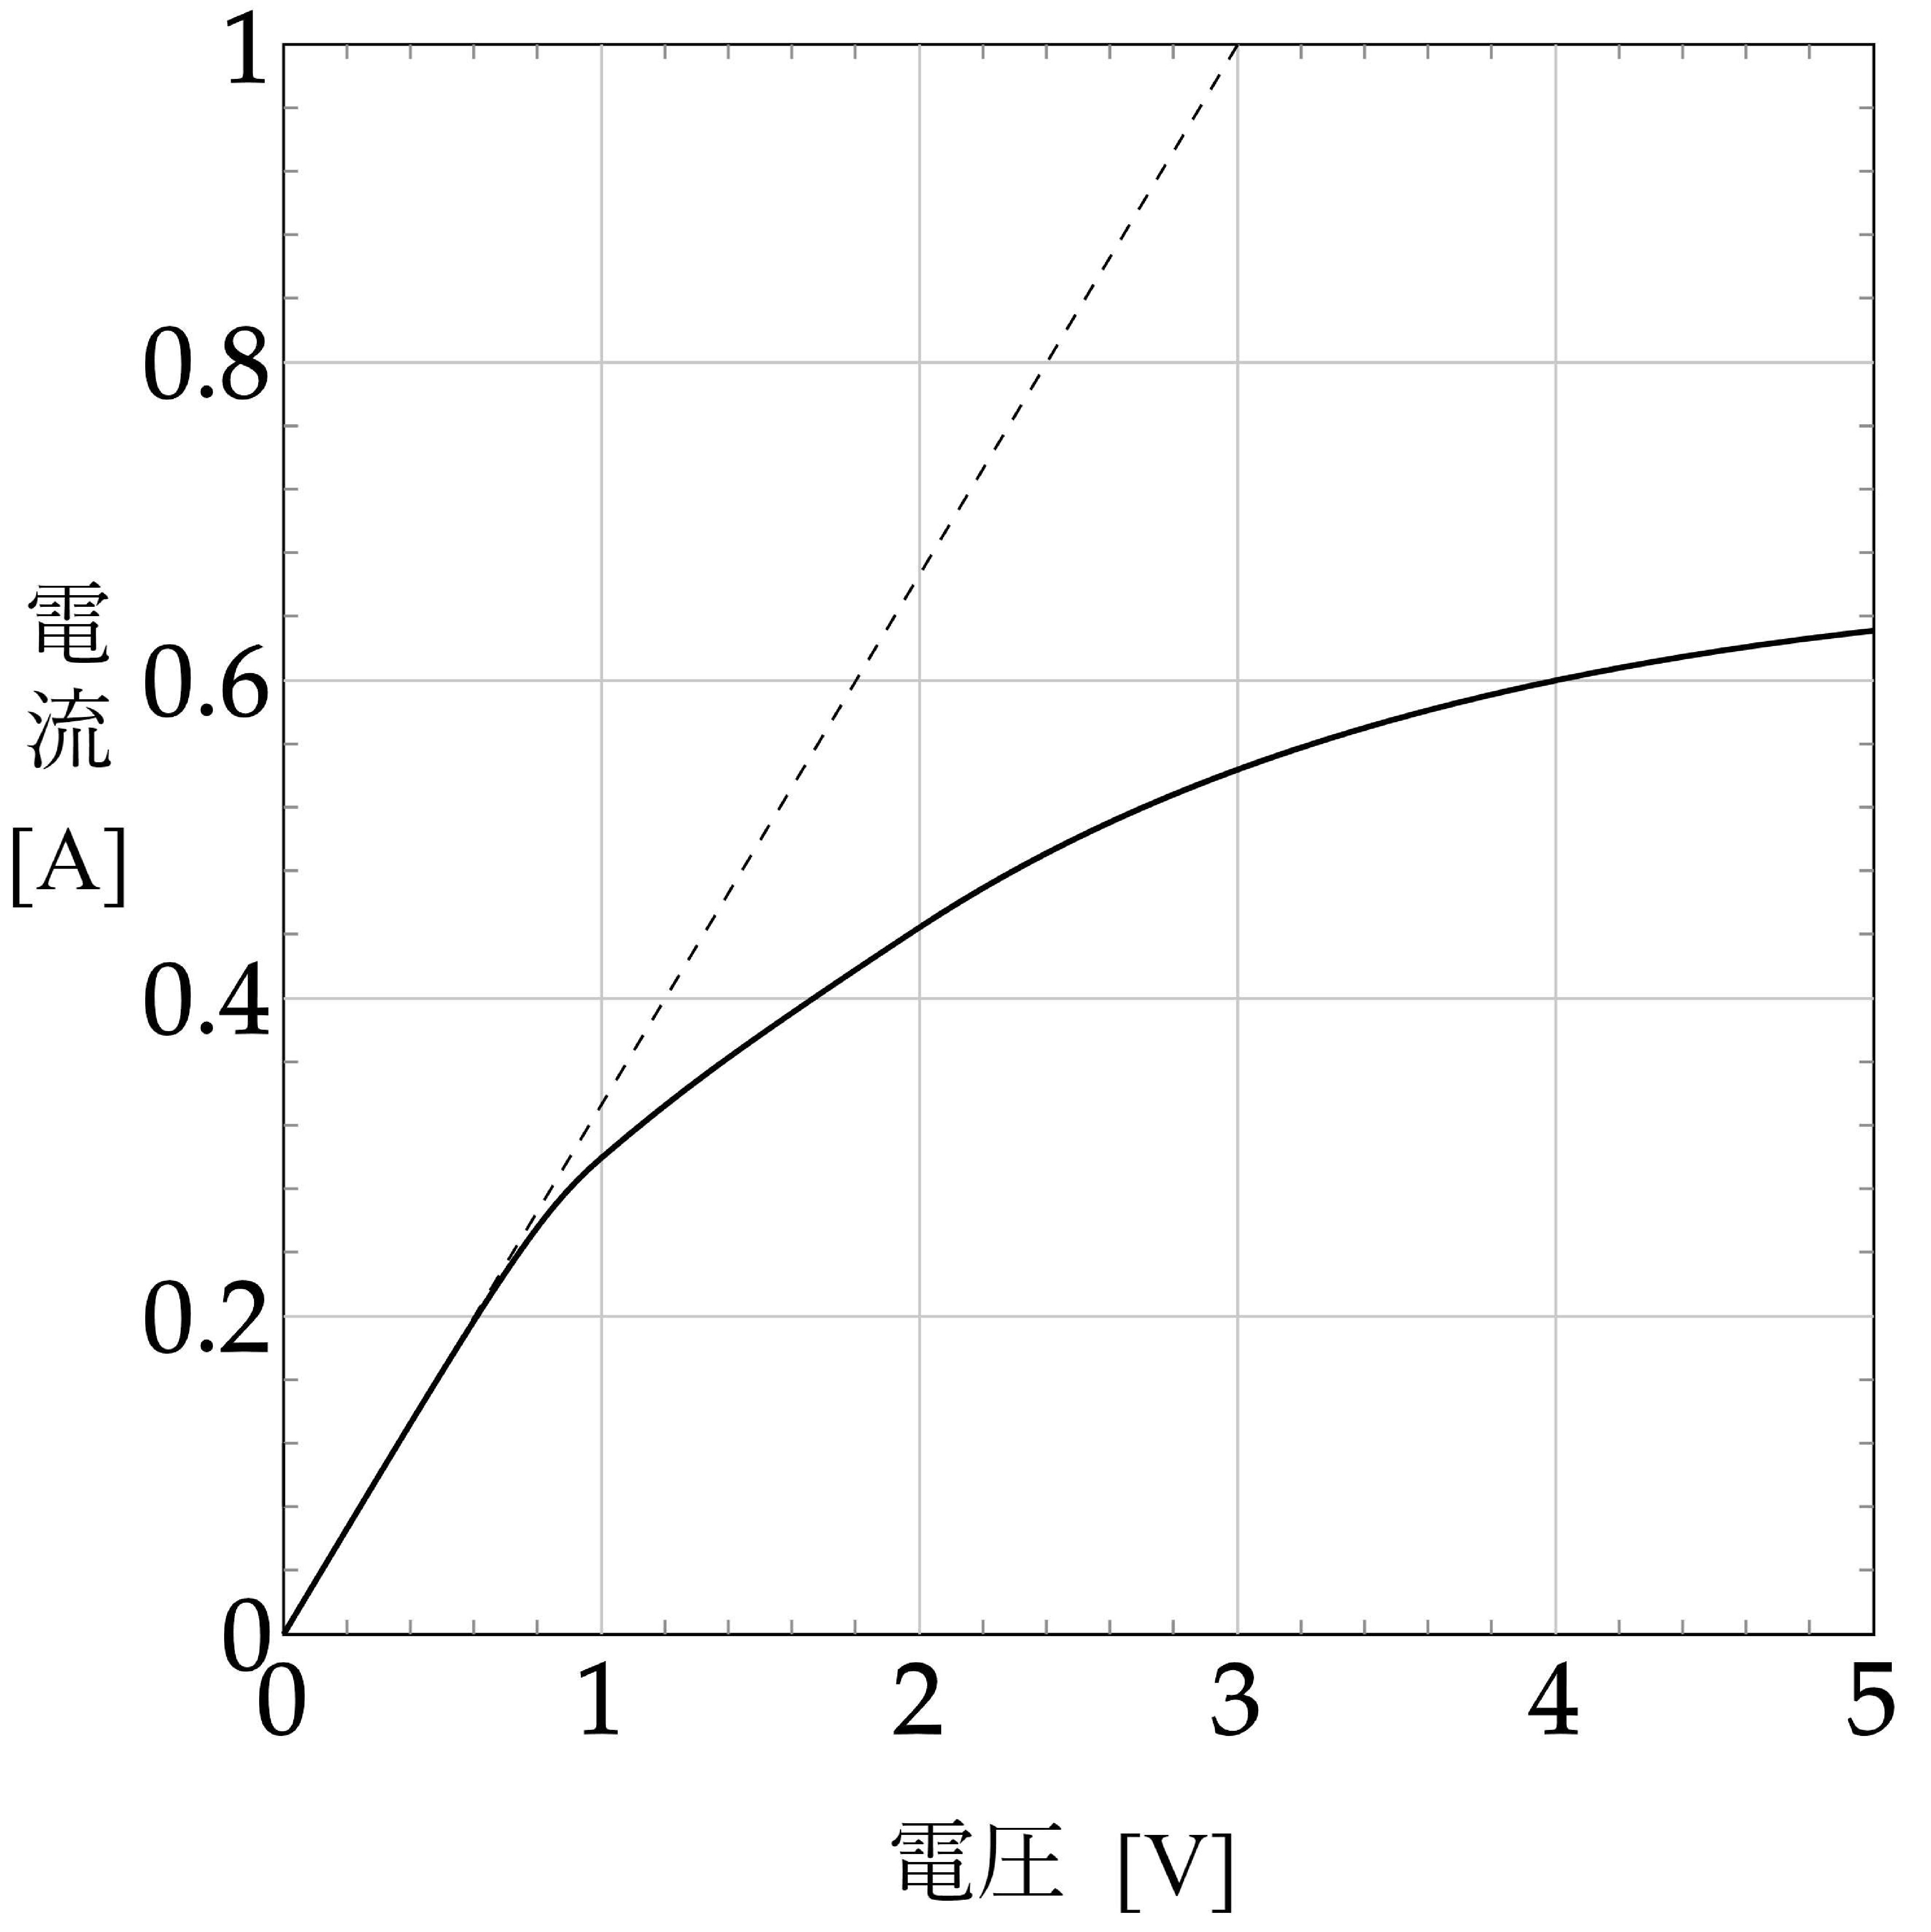
\includegraphics[width=6cm]{fig/fig_4_11_2.pdf}
    \caption{}
  \end{figure}
\end{minipage}



\begin{enumerate}[label={問\arabic*}]
  \item 電球の電流・電圧特性が図2のように,直線からずれる理由を60字程度で説明せよ.
  \item スイッチを入れた直後における回路全体の抵抗値$R_X$〔$\Omega$〕を求め,そのとりうる範囲を求めよ.ここで,可変抵抗の値は$R$〔$\Omega$〕で,その大きさは0から無限に大きな値まで変えられるものとする.
  \item 問2において,3つの電球と可変抵抗で消費される電力の総和$P$と$R_X$との関係を求めよ.また,その概略をグラフで示せ.
  \item 問3で求めた$P$の最大値について考察せよ.
  \item スイッチを入れてから十分に時間が経過すると,3つの電球の明るさが同じになった.そのときの$R_X$を求めよ.ただし,$r = 2$〔$\Omega$〕とする.

\end{enumerate}

\end{document}
